Considerando a influência do cross-pitch e cross-yaw, e implementando o desacoplamento, obtemos um diagrama de controle correspondente a figura \ref{fig:ControleMIMOPID}. Para um sistema já desacoplado, resta realizar o controle isolado de cada grandeza a ser controlada da planta.

\begin{figure}[H]
    \centering
    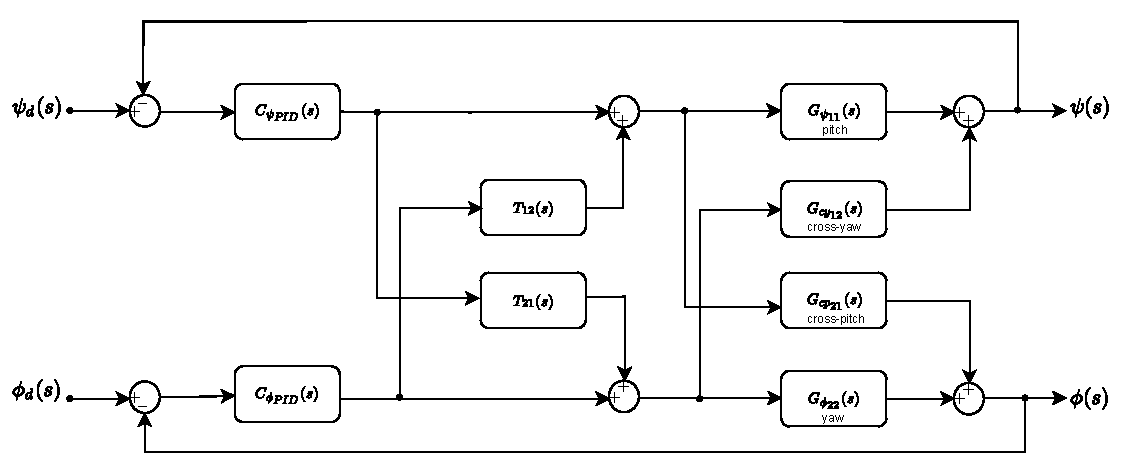
\includegraphics[width=0.48\textwidth]{figures/Controle/Controle_PID_Desacoplado.pdf}
    \caption{Diagrama de blocos do sistema MIMO com desacopladores e controladores PID para o \textit{yaw} e o \textit{pitch}.}
    \label{fig:ControleMIMOPID}
\end{figure}


Para realizar o controle de arfagem e guinada, projetou-se, por meio dos método do lugar das raízes, um controlador, seguindo os requisitos de desempenho apresentados na seção 2. O ganho foi ajustado iterativamente de forma a reduzir a ação de controle, via simulações, para que esta não atinja a saturação de 2.5V.
As figuras \ref{fig:rLocusPitch} e  \ref{fig:rLocusYaw} apresentam o lugar das raízes do PID para o controle de pitch e de yaw.

\begin{figure}[H]
    \centering
    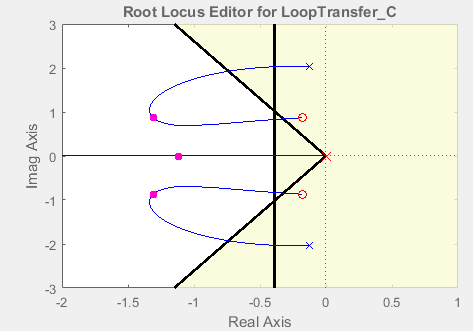
\includegraphics[width=0.48\textwidth]{figures/rlocus_MF.PNG}
    \caption{Lugar das raízes de um controlador PID para o controle do  \textit{pitch}.}
    \label{fig:rLocusPitch}
\end{figure}

\begin{figure}[H]
    \centering
    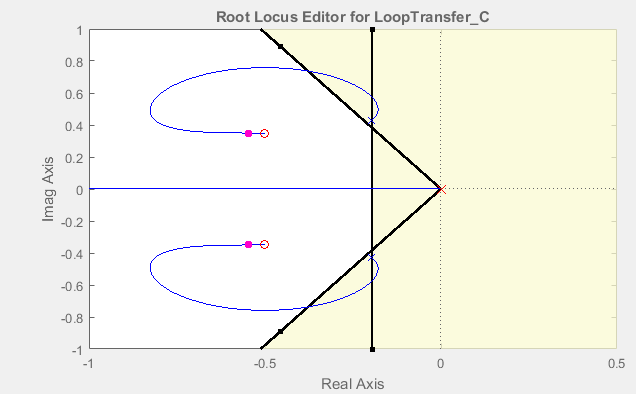
\includegraphics[width=0.48\textwidth]{figures/controlador_yaw_root_locus.PNG}
    \caption{Lugar das raízes de um controlador PID para o controle do  \textit{pitch}.}
    \label{fig:rLocusYaw}
\end{figure}


O controlador PID obtido para o pitch é dado pela equação \eqref{eq:PIDpitch}
\begin{equation}\label{eq:PIDpitch}
    C(s) = \frac{1.8 s^2 + 0.648 s + 0.789}{s}
\end{equation}


O controlador PID obtido para o yaw é dado pela equação \eqref{eq:PIDyaw}
\begin{equation}\label{eq:PIDyaw}
    C(s) = \frac{6.13 s^2 + 6.13 s + 3}{s}
\end{equation}